\documentclass[11pt,a4paper]{article}

% ---------------------------------------------------------------
%  EDIT THESE THREE LINES BEFORE SUBMITTING
% ---------------------------------------------------------------
\newcommand{\studentname}{Boralugoda M.S.}          % full name
\newcommand{\indexno}{220074B}             % index number
\newcommand{\subdate}{\today}              % submission date
\newcommand{\codeurl}{https://github.com/msboralugoda/EN3330-Assignment-3.git}  
% ---------------------------------------------------------------

\usepackage[margin=2.5cm]{geometry}
\IfFileExists{lmodern.sty}{\usepackage[T1]{fontenc}\usepackage{lmodern}}{}
\usepackage{amsmath,amssymb,amsthm}
\usepackage{booktabs}
\usepackage{caption,subcaption}
\usepackage{enumitem}
\usepackage{xcolor}
\usepackage{graphicx}
\usepackage{needspace}
\usepackage{tcolorbox}
\usepackage{fancyhdr}
\usepackage[hidelinks]{hyperref}
\usepackage{setspace}
\onehalfspacing

\definecolor{c0}{HTML}{1F77B4}
\definecolor{c1}{HTML}{FF7F0E}
\definecolor{c2}{HTML}{2CA02C}
\definecolor{c3}{HTML}{D62728}
\definecolor{c4}{HTML}{9467BD}
\definecolor{c5}{HTML}{8C564B}

\newtcolorbox{result}{colback=blue!4,colframe=blue!40!black,boxrule=0.5pt,arc=2pt,left=6pt,right=6pt,top=4pt,bottom=4pt}

\pagestyle{fancy}
\fancyhf{}
\lhead{EN3330 -- Assignment 03}
\rhead{\indexno}
\cfoot{\thepage}
\setlength{\headheight}{14pt}

\newcommand{\Lag}{\mathcal{L}}

\begin{document}

% ======================= TITLE PAGE ============================
\begin{titlepage}
  \centering
  \vspace*{2cm}
  {\Large University of Moratuwa\par}
  \vspace{0.3cm}
  {\large Department of Electronic and Telecommunication Engineering\par}
  \vspace{1.5cm}
  
\includegraphics[width=0.32\textwidth]{figures/uom_logo.png}\par
  \vspace{1.2cm}
  {\Large\bfseries EN3330\par}
  \vspace{0.5cm}
  {\huge\bfseries Assignment 03\par}
  \vspace{0.4cm}
  {\Large Lagrangian Duality, Saddle Points and Weak Duality\par}
  \vspace{1.5cm}
  \begin{tabular}{rl}
    \textbf{Name:} & \studentname \\[4pt]
    \textbf{Index No:} & \indexno \\[4pt]
    \textbf{Date:} & \subdate \\
  \end{tabular}
  \vfill
\end{titlepage}

% ======================= QUESTION 1 ============================
\section*{Problem Setup}
Throughout, we study
\begin{equation}
  \min_x\; f(x)=x^2 \quad \text{subject to}\quad h(x)=1-x\le 0,
\end{equation}
with Lagrangian $\Lag(\mu,x)=x^2+\mu(1-x)$, $\mu\ge 0$. The feasible set is $[1,\infty)$. Since $f$ is increasing on that set, the primal optimum is $x^\ast=1$ with $p^\ast=f(1)=1$; the unconstrained minimiser $x=0$ is infeasible, so the constraint must be active at the optimum.

\subsection*{Source Code}
All figures in this report were generated in Python (NumPy, Matplotlib) by the script \path{en3330_a03_plots.py}. The script also prints the numerical checks quoted in the text (e.g.\ a brute-force minimisation of $\Lag(\mu,\cdot)$ over a fine grid to confirm the analytical $d(\mu)$). The code is available at:
\begin{center}\url{\codeurl}\end{center}

\section{Question 1}

\subsection{(a) The Lagrangian as a function of $x$}

For fixed $\mu$, $\Lag(\mu,\cdot)$ is a convex parabola in $x$. Setting the derivative to zero,
\begin{equation}
  \frac{\partial \Lag}{\partial x}=2x-\mu=0 \;\Longrightarrow\; x(\mu)=\frac{\mu}{2},
  \qquad \frac{\partial^2 \Lag}{\partial x^2}=2>0,
\end{equation}
so $x(\mu)=\mu/2$ is the unique global minimiser, with minimum value $\Lag(\mu,x(\mu))=\mu-\mu^2/4$.

\begin{table}[h]
  \centering
  \begin{tabular}{cccc}
    \toprule
    $\mu$ & $\Lag(\mu,x)$ & $x(\mu)=\mu/2$ & $\min_x \Lag(\mu,x)$ \\
    \midrule
    0 & $x^2$         & 0   & 0    \\
    1 & $x^2-x+1$     & 0.5 & 0.75 \\
    2 & $x^2-2x+2$    & 1   & 1    \\
    3 & $x^2-3x+3$    & 1.5 & 0.75 \\
    \bottomrule
  \end{tabular}
  \caption{Lagrangian curves and their minimisers for $\mu=0,1,2,3$.}
  \label{tab:minimisers}
\end{table}

\begin{figure}[h]
  \centering
  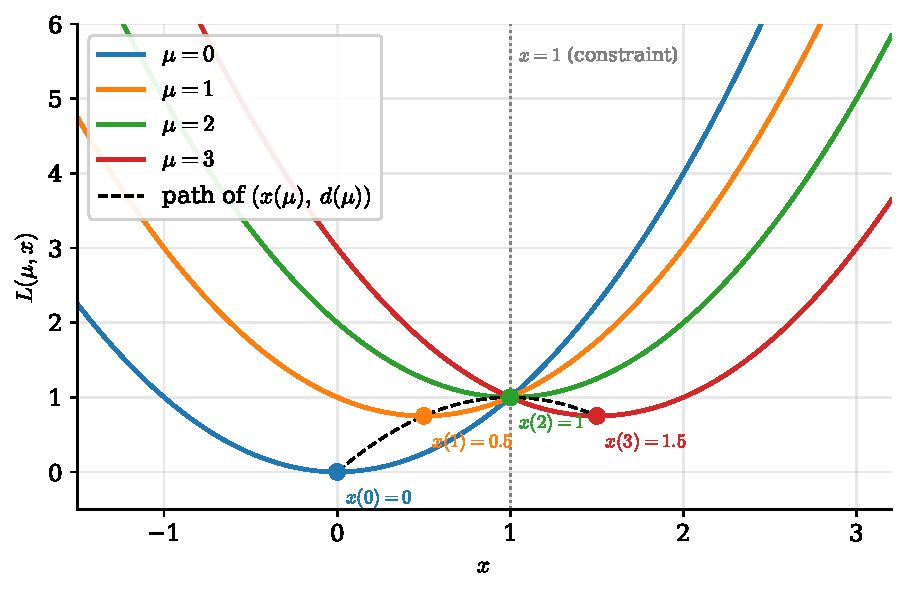
\includegraphics[width=0.85\textwidth]{figures/q1a_lagrangian_vs_x.pdf}
  \caption{$\Lag(\mu,x)$ versus $x$ for $\mu=0,1,2,3$. Dots mark the minimisers $x(\mu)=\mu/2$; the dashed curve is the locus $\bigl(x,\,2x-x^2\bigr)$ traced by the minimum point as $\mu$ varies.}
  \label{fig:q1a}
\end{figure}

\needspace{5\baselineskip}
\subsubsection*{Discussion}
Adding $\mu(1-x)$ tilts the parabola $x^2$ by a straight line of slope $-\mu$. Increasing $\mu$ therefore pushes the minimiser to the right linearly, $x(\mu)=\mu/2$, i.e.\ towards (and eventually beyond) the feasible region $x\ge 1$. The multiplier acts as a \emph{price} for violating the constraint: at $\mu=0$ the constraint is ignored and the minimiser $x=0$ is infeasible; at $\mu=1$ it is still infeasible; at $\mu=2$ the minimiser lands exactly on the boundary $x=1$; and at $\mu=3$ the penalty ``over-pays'', pushing the minimiser to $x=1.5$, which is feasible but not optimal for the original problem. The minimum value $\min_x\Lag$ first rises and then falls, peaking at $\mu=2$ --- a first sign that $\mu=2$ is special. Note also that every curve passes through the point $(1,1)$: since $h(1)=0$, the penalty term vanishes on the constraint boundary regardless of $\mu$, a fact used again in Q2.

\subsection{(b) The dual function}

Substituting $x(\mu)=\mu/2$ into the Lagrangian,
\begin{equation}
  d(\mu)=\Lag\!\left(\mu,\tfrac{\mu}{2}\right)=\frac{\mu^2}{4}+\mu-\frac{\mu^2}{2}
  =\boxed{\,\mu-\frac{\mu^2}{4}\,},\qquad \mu\ge 0.
\end{equation}
This is a concave parabola. Maximising over $\mu\ge 0$:
\begin{equation}
  d'(\mu)=1-\frac{\mu}{2}=0\;\Longrightarrow\;\mu^\ast=2\;(\ge 0,\ \text{so admissible}),\qquad d''(\mu)=-\tfrac12<0.
\end{equation}

\begin{result}
  \centering
  $\mu^\ast=2,\qquad d^\ast=d(2)=2-1=1.$
\end{result}
\noindent A numerical check in the script confirms this: minimising $\Lag(\mu,x)$ by brute force over a fine $x$-grid reproduces $d(\mu)$ to four decimal places at $\mu=0,1,2,3$, and a grid search over $\mu\in[0,10]$ returns $\mu^\ast=2.000$, $d^\ast=1.0000$.

\begin{figure}[h]
  \centering
  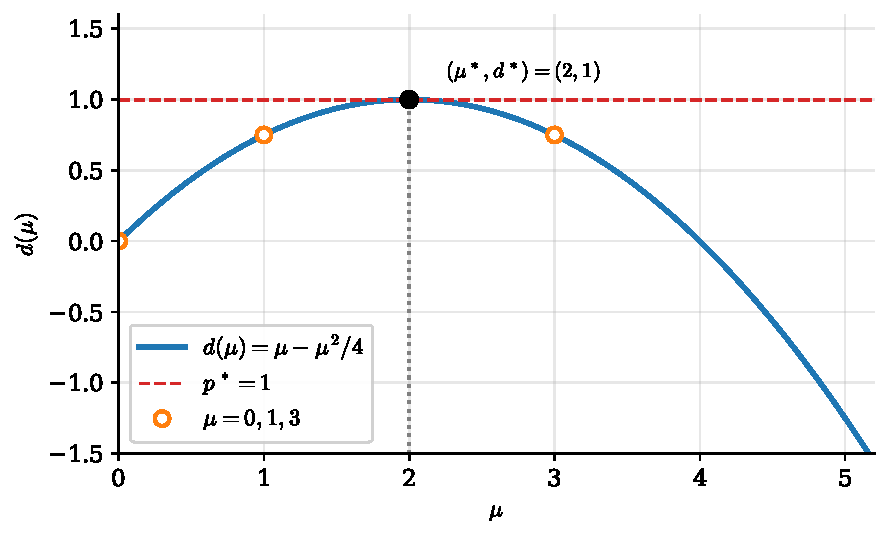
\includegraphics[width=0.75\textwidth]{figures/q1b_dual_function.pdf}
  \caption{Dual function $d(\mu)$. It is concave, maximised at $\mu^\ast=2$, and touches the primal optimal value $p^\ast=1$ there. The hollow markers are the values from Table~\ref{tab:minimisers}.}
  \label{fig:q1b}
\end{figure}

\needspace{5\baselineskip}
\subsubsection*{Discussion}
The dual function is concave (as it must be, see Q3(b)), and its maximum $d^\ast=1$ coincides with the primal optimum $p^\ast=1$: there is \emph{zero duality gap} (strong duality). This is expected here because the problem is convex ($f$ convex, $h$ affine) and Slater's condition holds (e.g.\ $x=2$ gives $h(2)=-1<0$). Note also $x(\mu^\ast)=1=x^\ast$: at the optimal price, the unconstrained minimiser of the Lagrangian recovers the constrained primal solution.

\subsection{(c) The primal function}

For fixed $x$, $\Lag(\mu,x)=x^2+\mu(1-x)$ is an \emph{affine} function of $\mu$ with slope $1-x=h(x)$. Hence, splitting into feasible ($x\ge1$) and infeasible ($x<1$) points,
\begin{equation}
  g(x)=\max_{\mu\ge0}\bigl[x^2+\mu(1-x)\bigr]=
  \begin{cases}
    x^2, & x\ge1 \text{ (slope}\le 0\text{, so }\mu=0\text{ is best)},\\[2pt]
    +\infty, & x<1 \text{ (slope}>0\text{, let }\mu\to\infty).
  \end{cases}
\end{equation}

Figure~\ref{fig:q1c} demonstrates this graphically: we plot $\Lag(\mu,x)$ on $x\in[-1,3]$ for a growing sequence of $\mu$. Their pointwise maximum is $g(x)$. In the script, $g(x)$ is approximated numerically as the maximum of $\Lag(\mu,x)$ over $\mu\in[0,10^4]$: for $x\ge1$ this returns $x^2$, while for $x<1$ it grows with the upper end of the $\mu$-range, as expected for $+\infty$.

\begin{figure}[h]
  \centering
  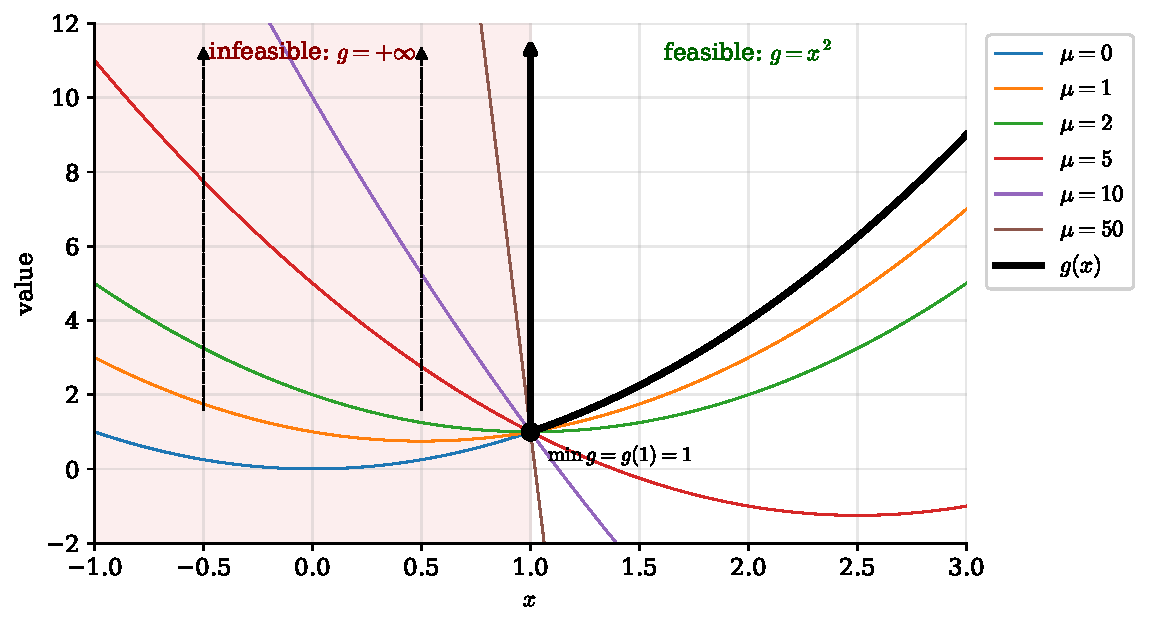
\includegraphics[width=0.9\textwidth]{figures/q1c_primal_function.pdf}
  \caption{Primal function $g(x)=\max_{\mu\ge0}\Lag(\mu,x)$ (thick black). For $x<1$ the curves increase without bound as $\mu$ grows (arrows), so $g=+\infty$. For $x\ge1$ every curve lies on or below $x^2$ (for $x>1$ larger $\mu$ pulls the curve \emph{down}), and the $\mu=0$ curve attains it, so $g(x)=x^2$.}
  \label{fig:q1c}
\end{figure}

\paragraph{Why $\min_x g(x)$ is equivalent to problem (1).} The function $g$ acts as an exact ``infinite barrier'': it agrees with the objective $f(x)=x^2$ on the feasible set and is $+\infty$ everywhere else,
\[
  g(x)=f(x)+I_{\{x\ge1\}}(x),\qquad I_{C}(x)=\begin{cases}0,&x\in C\\ +\infty,&x\notin C.\end{cases}
\]
Any minimiser of $g$ can never lie in the infeasible region (it would have infinite cost while feasible points have finite cost), and on the feasible region minimising $g$ is exactly minimising $f$. Hence
\[
  \min_x g(x)=\min_{x\ge1}x^2 = 1,\quad \text{attained at } x^\ast=1,
\]
the same optimal value and the same optimal point as problem (1). The constrained problem has been rewritten as the unconstrained \emph{min--max} problem $\min_x\max_{\mu\ge0}\Lag(\mu,x)$; the dual problem is obtained by swapping the order, $\max_{\mu\ge0}\min_x\Lag(\mu,x)$.

% ======================= QUESTION 2 ============================
\section{Question 2}

\subsection{(a) $(x^\ast,\mu^\ast)=(1,2)$ is a saddle point}

\paragraph{(i)} $\Lag(\mu^\ast,x^\ast)=\Lag(2,1)=1^2+2(1-1)=\boxed{1}$.

\paragraph{(ii)} For any $\mu\ge0$,
\[
  \Lag(\mu,x^\ast)=1^2+\mu(1-1)=1,
\]
which is independent of $\mu$ because $h(x^\ast)=0$ (the constraint is active). Therefore
$\Lag(\mu,x^\ast)=1\le1=\Lag(\mu^\ast,x^\ast)$ for all $\mu\ge0$; the left inequality holds (with equality).

\paragraph{(iii)} With $\mu^\ast=2$,
\[
  \Lag(\mu^\ast,x)=x^2+2(1-x)=x^2-2x+1+1=(x-1)^2+1.
\]
Since $(x-1)^2\ge0$ for every $x$, $\Lag(\mu^\ast,x)\ge1=\Lag(\mu^\ast,x^\ast)$ for all $x\in\mathbb{R}$, with equality only at $x=1$. The right inequality holds.

\begin{result}
  \centering
  $\Lag(\mu,x^\ast)=1\;\le\;\Lag(\mu^\ast,x^\ast)=1\;\le\;\Lag(\mu^\ast,x)=(x-1)^2+1\qquad \forall\mu\ge0,\ \forall x.$
\end{result}

\paragraph{(iv)} Plots are shown in Figure~\ref{fig:q2a}.

\begin{figure}[h]
  \centering
  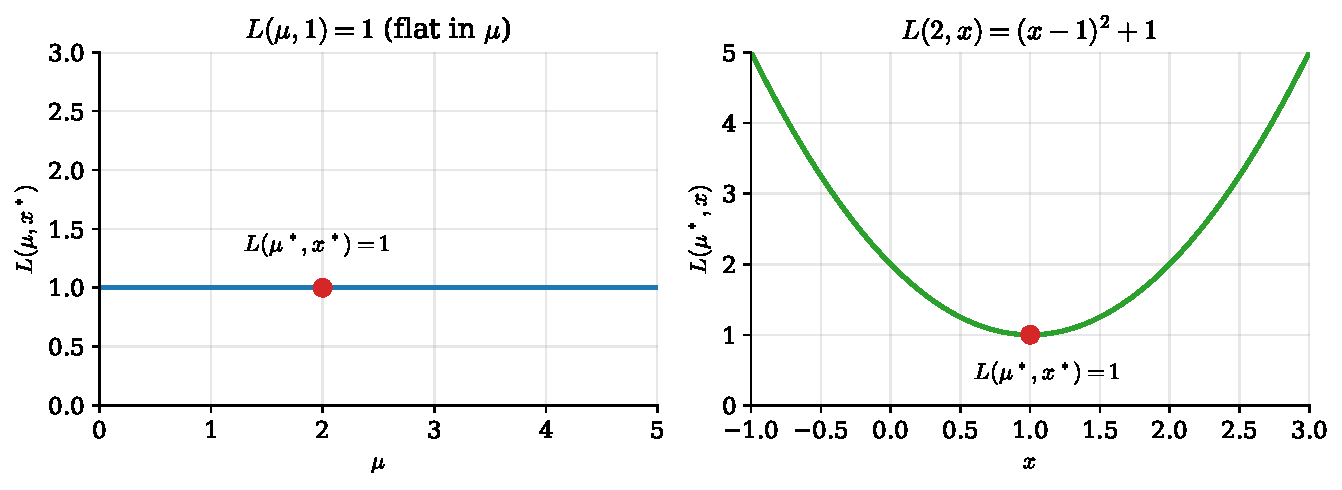
\includegraphics[width=\textwidth]{figures/q2a_saddle_slices.pdf}
  \caption{The two slices of $\Lag$ through $(\mu^\ast,x^\ast)=(2,1)$. Left: $\Lag(\mu,1)=1$ is flat in $\mu$, so it is (weakly) maximised at $\mu^\ast=2$. Right: $\Lag(2,x)=(x-1)^2+1$ is minimised at $x^\ast=1$. Along $\mu$ the point is a maximum, along $x$ it is a minimum --- the defining property of a saddle point.}
  \label{fig:q2a}
\end{figure}

\needspace{5\baselineskip}
\subsubsection*{Discussion}
Along the $x$-direction, $(x^\ast,\mu^\ast)$ is a minimum; along the $\mu$-direction it is a maximum. Hence neither ``player'' can improve by deviating unilaterally: the primal player (minimising over $x$) cannot lower $\Lag$ given $\mu^\ast$, and the dual player (maximising over $\mu$) cannot raise it given $x^\ast$. The existence of such a saddle point is equivalent to $\min_x\max_\mu\Lag=\max_\mu\min_x\Lag$, i.e.\ to strong duality, which agrees with $p^\ast=d^\ast=1$ found in Q1. Note that the maximum in $\mu$ is not strict --- every $\mu\ge0$ ties --- because the constraint is exactly active at $x^\ast$.

\subsection{(b) The optimality chain}

For any feasible $x$ (i.e.\ $h(x)\le0$):
\[
  f(x^\ast)\overset{(1)}{=}\Lag(\mu^\ast,x^\ast)\overset{(2)}{\le}\Lag(\mu^\ast,x)\overset{(3)}{=}f(x)+\mu^\ast h(x)\overset{(4)}{\le}f(x).
\]
\begin{enumerate}[label=(\arabic*), leftmargin=2em]
  \item $\Lag(\mu^\ast,x^\ast)=f(x^\ast)+\mu^\ast h(x^\ast)$ and $\mu^\ast h(x^\ast)=0$ by complementary slackness (here $2\cdot 0=0$).
  \item This is the right saddle-point inequality: $x^\ast$ minimises $\Lag(\mu^\ast,\cdot)$ over all $x$.
  \item By the definition of the Lagrangian, $\Lag(\mu,x)=f(x)+\mu h(x)$.
  \item $\mu^\ast\ge0$ and $h(x)\le0$ for feasible $x$, so $\mu^\ast h(x)\le0$.
\end{enumerate}
Since $f(x^\ast)\le f(x)$ for every feasible $x$, $x^\ast$ is primal optimal. (For our problem: $1\le (x-1)^2+1 = x^2+2(1-x)\le x^2$ for all $x\ge1$.)

\paragraph{What the left inequality says about $h(x^\ast)$.} The left inequality reads
\[
  \Lag(\mu,x^\ast)=f(x^\ast)+\mu\,h(x^\ast)\le\Lag(\mu^\ast,x^\ast)<\infty\qquad\forall\mu\ge0.
\]
The left side is affine in $\mu$ with slope $h(x^\ast)$. If $h(x^\ast)>0$ it would grow without bound as $\mu\to\infty$, contradicting the finite upper bound. Therefore
\[
  h(x^\ast)\le0,
\]
i.e.\ the left inequality \emph{forces primal feasibility} of $x^\ast$. Moreover, setting $\mu=0$ in the left inequality gives $f(x^\ast)\le f(x^\ast)+\mu^\ast h(x^\ast)$, i.e.\ $\mu^\ast h(x^\ast)\ge0$; combined with $\mu^\ast\ge0$ and $h(x^\ast)\le0$ this yields $\mu^\ast h(x^\ast)=0$. So the left inequality also implies \emph{complementary slackness}, which is exactly what step (1) used. In our problem $h(x^\ast)=0$, which is why $\Lag(\mu,x^\ast)$ was flat in $\mu$.

\subsection{(c) Complementary slackness and an inactive constraint}

\paragraph{Original problem.} $\mu^\ast h(x^\ast)=2\cdot(1-1)=2\cdot0=0$. \checkmark\ The condition holds because the constraint is \emph{active} ($h(x^\ast)=0$), which allows a strictly positive multiplier.

\paragraph{Modified constraint $x\ge-1$.} Now $h(x)=-1-x\le0$.
\begin{itemize}
  \item \textbf{Feasibility:} the unconstrained minimiser $x=0$ satisfies $0\ge-1$, so it is feasible. It is therefore also the constrained optimum: $x^\ast=0$, $p^\ast=0$.
  \item \textbf{Activity:} $h(0)=-1<0$, so the constraint is \emph{inactive} (strictly satisfied); it does not influence the solution.
  \item \textbf{Expected multiplier:} complementary slackness $\mu^\ast h(x^\ast)=\mu^\ast(-1)=0$ forces $\boxed{\mu^\ast=0}$. Intuitively, the multiplier is the marginal value (``shadow price'') of the constraint; a constraint that is not binding is worth nothing, since perturbing it slightly does not change the optimum.
\end{itemize}

\paragraph{Verification.} $\Lag(\mu,x)=x^2+\mu(-1-x)$ is minimised at $x(\mu)=\mu/2$, giving
\[
  d(\mu)=\frac{\mu^2}{4}-\mu-\frac{\mu^2}{2}=-\mu-\frac{\mu^2}{4},
\]
which is strictly decreasing on $\mu\ge0$, so $\mu^\ast=0$ and $d^\ast=d(0)=0=p^\ast$. The left saddle inequality now reads $\Lag(\mu,0)=-\mu\le0=\Lag(0,0)$, which holds for all $\mu\ge0$ and is strict for $\mu>0$: any positive price on a slack constraint strictly lowers $\Lag$ at $x^\ast$, so the maximising dual variable must be zero.

\begin{figure}[h]
  \centering
  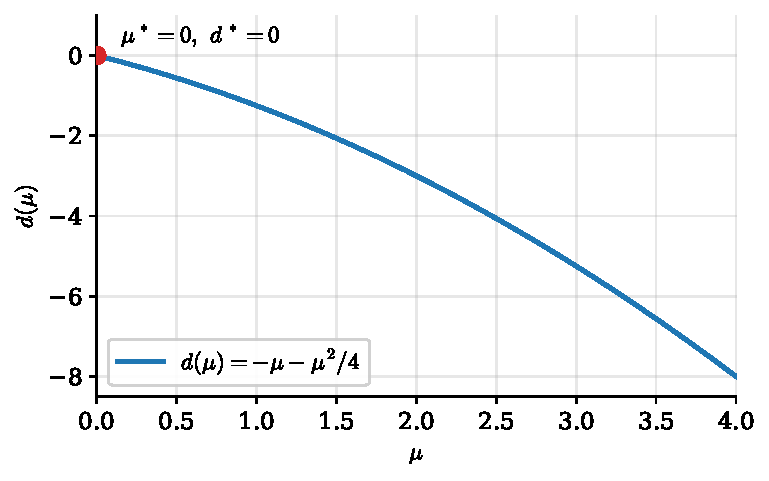
\includegraphics[width=0.6\textwidth]{figures/q2c_dual_inactive.pdf}
  \caption{Dual function for the constraint $x\ge-1$. Its maximum over $\mu\ge 0$ is at the boundary $\mu^\ast=0$.}
  \label{fig:q2c}
\end{figure}

% ======================= QUESTION 3 ============================
\section{Question 3: Weak Duality}

\subsection{(a) Proof and numerical check}

Let $\mu\ge0$ and let $x$ be feasible ($h(x)\le0$). Then
\[
  d(\mu)\overset{(1)}{\le}\Lag(\mu,x)=f(x)+\mu h(x)\overset{(2)}{\le}f(x).
\]
\begin{enumerate}[label=(\arabic*), leftmargin=2em]
  \item $d(\mu)$ is the minimum of $\Lag(\mu,\cdot)$ over \emph{all} $x$, so it cannot exceed the value of $\Lag(\mu,\cdot)$ at any particular $x$ (feasible or not).
  \item $\mu\ge0$ and $h(x)\le0$, hence $\mu h(x)\le0$, so adding it to $f(x)$ cannot increase it.
\end{enumerate}
Thus $d(\mu)\le f(x)$ for \emph{every} feasible $x$, i.e.\ $d(\mu)$ is a lower bound on the objective over the feasible set. Taking the infimum over feasible $x$ on the right,
\[
  d(\mu)\le\inf_{h(x)\le0}f(x)=p^\ast\qquad\forall\mu\ge0,
\]
and in particular $d^\ast=\max_{\mu\ge0}d(\mu)\le p^\ast$. This is \textbf{weak duality}; it requires no convexity.

\paragraph{Numerical check for Q1} ($d(\mu)=\mu-\mu^2/4$, $p^\ast=1$):

\begin{table}[h]
  \centering
  \begin{tabular}{cccc}
    \toprule
    $\mu$ & $d(\mu)$ & $d(\mu)\le p^\ast=1$? & gap $p^\ast-d(\mu)$\\
    \midrule
    0 & $0$    & \checkmark & 1 \\
    1 & $0.75$ & \checkmark & 0.25 \\
    2 & $1$    & \checkmark (equality) & 0 \\
    3 & $0.75$ & \checkmark & 0.25 \\
    \bottomrule
  \end{tabular}
  \caption{Weak duality verified at $\mu=0,1,2,3$.}
\end{table}

In general $p^\ast-d(\mu)=1-\mu+\mu^2/4=(1-\mu/2)^2\ge0$, so the bound holds for every $\mu\ge0$, and it is tight only at $\mu=2$. Every choice of $\mu$ gives a valid lower bound on $p^\ast$; the dual problem searches for the best (largest) such bound.

\subsection{(b) $\Lag$ as a function of $\mu$ and the lower envelope}

For fixed $x$, $\Lag(\mu,x)=x^2+\mu(1-x)$ is a straight line in $\mu$ with intercept $f(x)=x^2$ and slope $h(x)=1-x$:
\[
  x=0:\ \Lag=\mu,\qquad x=1:\ \Lag=1,\qquad x=2:\ \Lag=4-\mu.
\]
Their lower envelope is
\[
  \tilde d(\mu)=\min\{\mu,\;1,\;4-\mu\}=
  \begin{cases}\mu,&0\le\mu\le1,\\ 1,&1\le\mu\le3,\\ 4-\mu,&\mu\ge3.\end{cases}
\]

\begin{figure}[h]
  \centering
  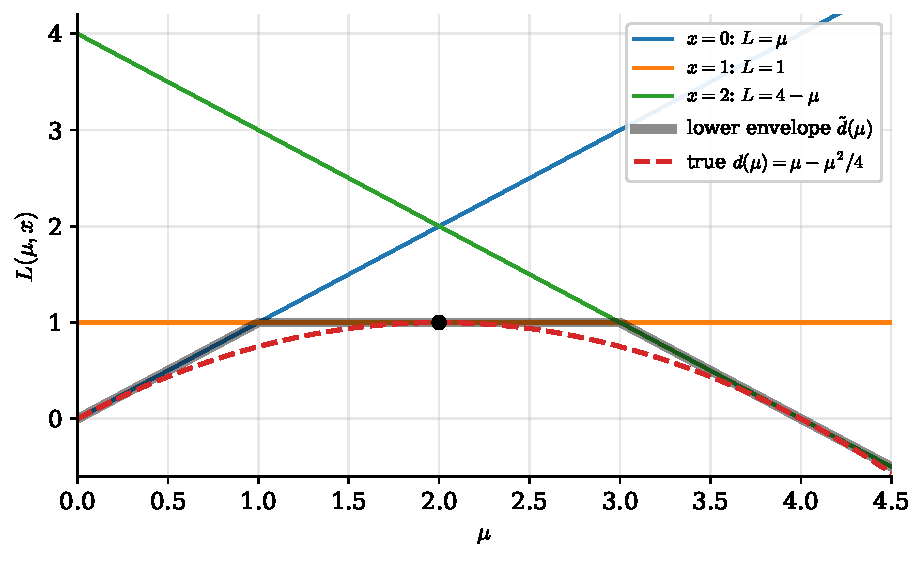
\includegraphics[width=0.8\textwidth]{figures/q3b_lower_envelope.pdf}
  \caption{$\Lag(\mu,x)$ versus $\mu$ for $x=0,1,2$ (straight lines), their lower envelope (thick grey), and the exact dual function (dashed). Including more values of $x$ adds more lines, and the envelope converges down to $d(\mu)$.}
  \label{fig:q3b}
\end{figure}

\needspace{5\baselineskip}
\subsubsection*{Discussion}
The envelope is \textbf{concave}: it is piecewise linear with slopes $1,\,0,\,-1$, i.e.\ non-increasing slopes. It lies above the true $d(\mu)$ because only three values of $x$ are used, and touches it where one of those $x$ is the actual minimiser ($\mu=0$ with $x=0$, $\mu=2$ with $x=1$, $\mu=4$ with $x=2$). Taking the minimum over all $x\in\mathbb{R}$ adds infinitely many tangent lines and yields the smooth concave curve $d(\mu)=\mu-\mu^2/4$.

\begin{result}
\textbf{Why $d$ is always concave.} For each fixed $x$, $\Lag(\mu,x)=f(x)+\mu h(x)$ is \emph{affine in $\mu$}, whatever $f$ and $h$ are, because $f(x)$ and $h(x)$ are just numbers. The dual function $d(\mu)=\min_x\Lag(\mu,x)$ is the pointwise minimum of a family of affine functions, and a pointwise minimum of affine functions is always concave --- so the dual problem is a concave maximisation even when $f$ is non-convex.
\end{result}

\end{document}
